\documentclass[11pt, a4paper]{article}
\usepackage[utf8]{inputenc}
\usepackage{graphicx}
\usepackage{blindtext}
\usepackage{booktabs} % For \toprule, \midrule and \bottomrule
\usepackage{pgfplotstable} % Generates table from .csv

% change default font family from serif to sans-serif
\renewcommand{\familydefault}{\sfdefault}

% change ToC, figure and table section titles to german equivalents
\renewcommand{\contentsname}{Inhaltsverzeichnis}
\renewcommand{\listfigurename}{Figuren- \& Abbildungsverzeichnis}
\renewcommand{\listtablename}{Tabellenverzeichnis}

\title{Projekttitel}
\date{2019-03-05}
\author{Projektdokumentation\\
       \\
       John Doe\\
       Awesome Denki - SuperElektrik GmbH\\
}

\begin{document}
  \pagenumbering{gobble}
  \maketitle
  \newpage

  \tableofcontents
  \newpage

  \pagenumbering{arabic}
  \begin{abstract}
  Short introduction to subject of the paper \ldots
  \end{abstract}
  \section{Definitionsphase}
    \subsection{Situationsanalyse}
   \blindtext

\subsection{Auftragsbeschreibung}
   \blindtext

\subsection{Problemdefinition}
   \blindtext

\subsection{Kundengespraech}
   \blindtext

\subsection{Ist-Analyse}
   \blindtext

\subsection{Soll-Konzept}
   \blindtext

\subsection{Projektziele}
\subsubsection{Terminziel}
\subsubsection{Kostenziel}


    \newpage

  \section{Planungsphase}
    \subsection{Projektstrukturplan}
   \blindtext
\subsection{Terminplan}
   \blindtext
\subsection{Kostenplan}
  \blindtext
\subsection{Qualitaetssicherungsplan}
  \blindtext
  \paragraph{Wartbarkeit}
  lorem ipsum dolor sit amet.
  \paragraph{Stabilitaet}
  lorem ipsum dolor sit amet.
  \paragraph{Performance}
  lorem ipsum dolor sit amet.
  \paragraph{Sorgfaeltige Planung}
  lorem ipsum dolor sit amet.
\subsection{Use Cases}
  \blindtext
\subsection{Domain Modelling und Klassendiagramme}
  \blindtext
\subsection{Datenbankmodel erstellen}
  \blindtext

    \newpage

  \section{Durchfuehrungsphase}
    \subsection{Use Cases}
  \blindtext
\subsection{Domain Modelling}
  \blindtext
\subsection{Datenbankentwurf}
  \blindtext
\subsection{GUI-Entwurf}
  \blindtext

    \newpage

  \section{Implementierungsphase}
    \subsection{Tests}
  \blindtext
  \subsubsection{Unit Tests}
  \subsubsection{Systemtests}
  \subsubsection{Bedienungstests}
\subsection{Quellcode}
  \blindtext
\subsection{Fachlicher Soll-Ist Vergleich}
  \blindtext
\subsection{Zeitlicher Soll-Ist Vergleich}
  \blindtext

    \newpage

    \pagenumbering{gobble}
    \begin{appendix}
      \listoffigures
      \listoftables
    \end{appendix}
    \newpage

  \section{Anhang: Figuren \& Tabellen}
    \pagenumbering{Roman}
    \subsection{Fragenkatalog zum Kundengespraech}
      \begin{table}[h!]
  \begin{center}
    \caption{Fragenkatalog zum Kundengespraech}
    \label{table1}
    \pgfplotstabletypeset[
      multicolumn names, % allows to have multicolumn names
      col sep=comma, % the seperator in our .csv file
      header=has colnames,
      columns={Fragen,Antworten},
      columns/Fragen/.style={column type={c|},string type},
      columns/Antworten/.style={column type={c|},string type},
      every head row/.style={
        before row={\toprule}, % have a rule at top
        after row={\midrule}
      },
      every last row/.style={
        after row=\bottomrule % rule at bottom
      }
    ]{csv/fragenkatalog.csv} % filename/path to file
  \end{center}
\end{table}

      \newpage

    \subsection{Projektstrukturplan}
      \begin{figure}[h!]
        \makebox[\textwidth]{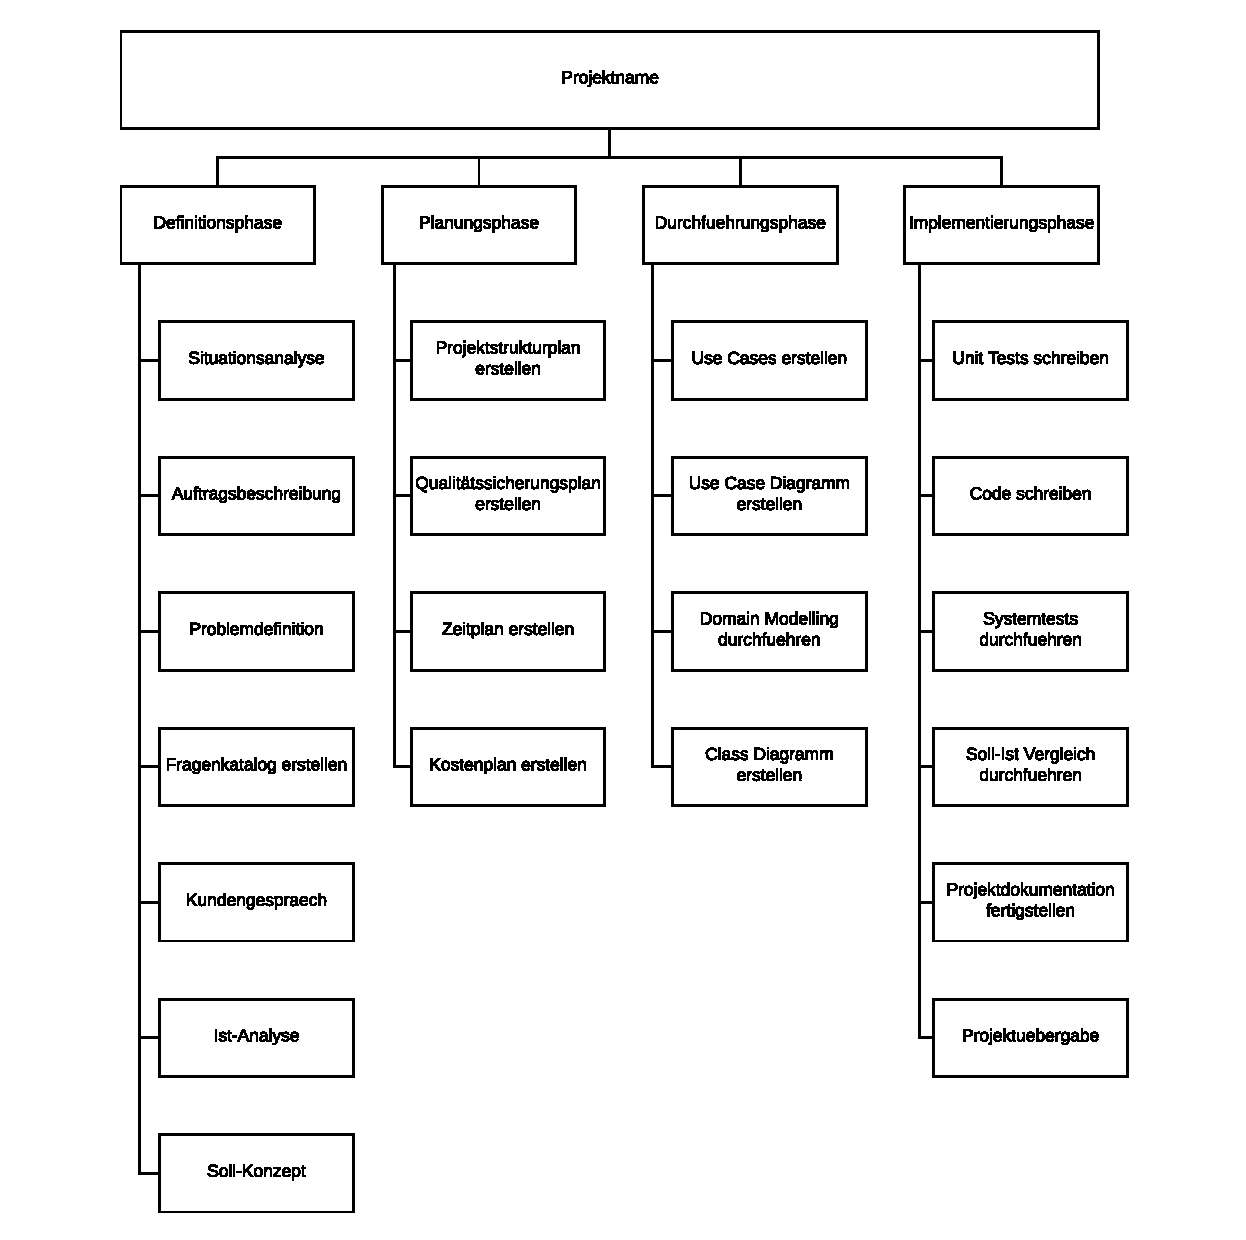
\includegraphics[width=1.4\linewidth]{fig/Projektstrukturplan.pdf}}
        \caption{Projektstrukturplan}
        \label{fig:psp}
      \end{figure}
      \newpage

    \subsection{Terminplan}
      \begin{table}[h!]
  \begin{center}
    \caption{Zeitplan}
    \label{table1}
    \pgfplotstabletypeset[
      multicolumn names, % allows to have multicolumn names
      col sep=comma, % the seperator in our .csv file
      header=has colnames,
      columns={Fragen,Antworten},
      columns/Fragen/.style={column type={c|},string type},
      columns/Antworten/.style={column type={c|},string type},
      every head row/.style={
        before row={\toprule}, % have a rule at top
        after row={\midrule}
      },
      every last row/.style={
        after row=\bottomrule % rule at bottom
      }
    ]{csv/zeitplan.csv} % filename/path to file
  \end{center}
\end{table}

      \newpage

    \subsection{Kostenplan}
      \begin{table}[h!]
  \begin{center}
    \caption{Kostenplan}
    \label{table1}
    \pgfplotstabletypeset[
      multicolumn names, % allows to have multicolumn names
      col sep=comma, % the seperator in our .csv file
      header=has colnames,
      columns={Fragen,Antworten},
      columns/Fragen/.style={column type={c|},string type},
      columns/Antworten/.style={column type={c|},string type},
      every head row/.style={
        before row={\toprule}, % have a rule at top
        after row={\midrule}
      },
      every last row/.style={
        after row=\bottomrule % rule at bottom
      }
    ]{csv/kostenplan.csv} % filename/path to file
  \end{center}
\end{table}

      \newpage

    \subsection{Qualitaetssicherungsplan}
      \begin{table}[h!]
  \begin{center}
    \caption{Qualitaetssicherungsplan}
    \label{table1}
    \pgfplotstabletypeset[
      multicolumn names, % allows to have multicolumn names
      col sep=comma, % the seperator in our .csv file
      header=has colnames,
      columns={Fragen,Antworten},
      columns/Fragen/.style={column type={c|},string type},
      columns/Antworten/.style={column type={c|},string type},
      every head row/.style={
        before row={\toprule}, % have a rule at top
        after row={\midrule}
      },
      every last row/.style={
        after row=\bottomrule % rule at bottom
      }
    ]{csv/qualitaetssicherungsplan.csv} % filename/path to file
  \end{center}
\end{table}

      \newpage

    \subsection{Use-Case Diagramm}
      \begin{figure}[h!]
        \makebox[\textwidth]{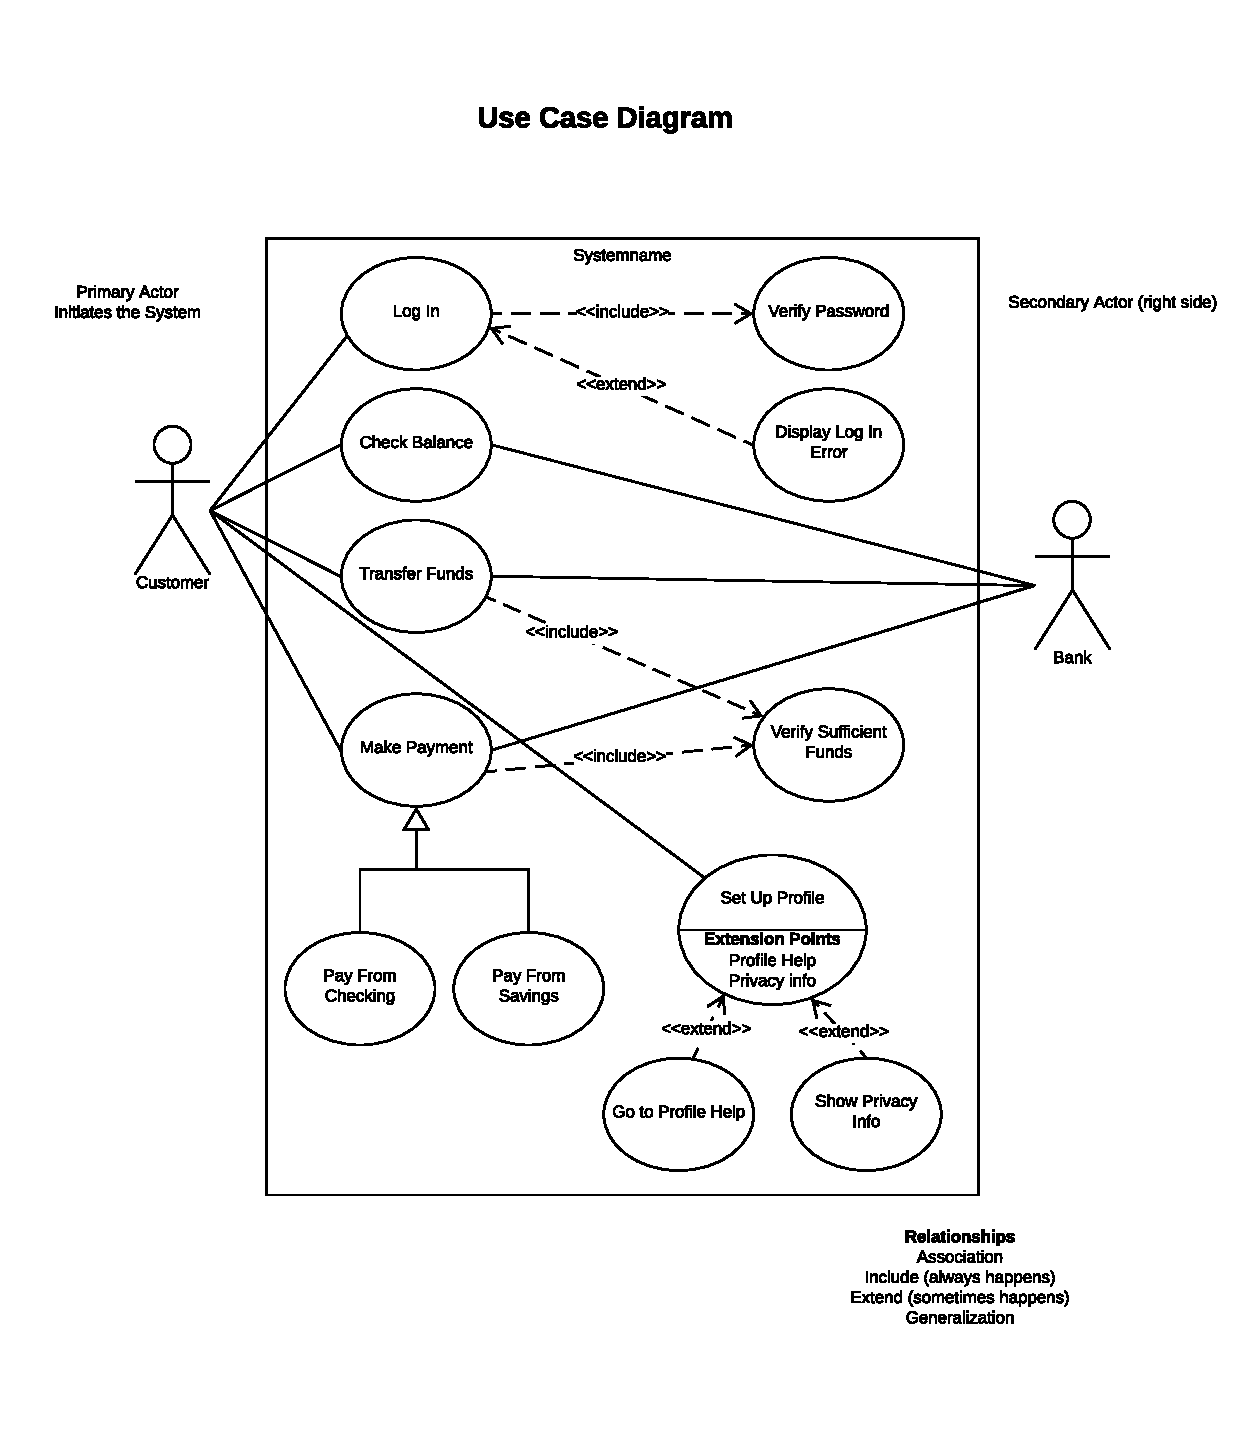
\includegraphics[width=1.2\linewidth]{fig/use_case_diagram.pdf}}
        \caption{Use Case Diagram}
        \label{fig:usecasediagram}
      \end{figure}
      \newpage

    \subsection{Klassendiagramm}
      \begin{figure}[h!]
        \makebox[\textwidth]{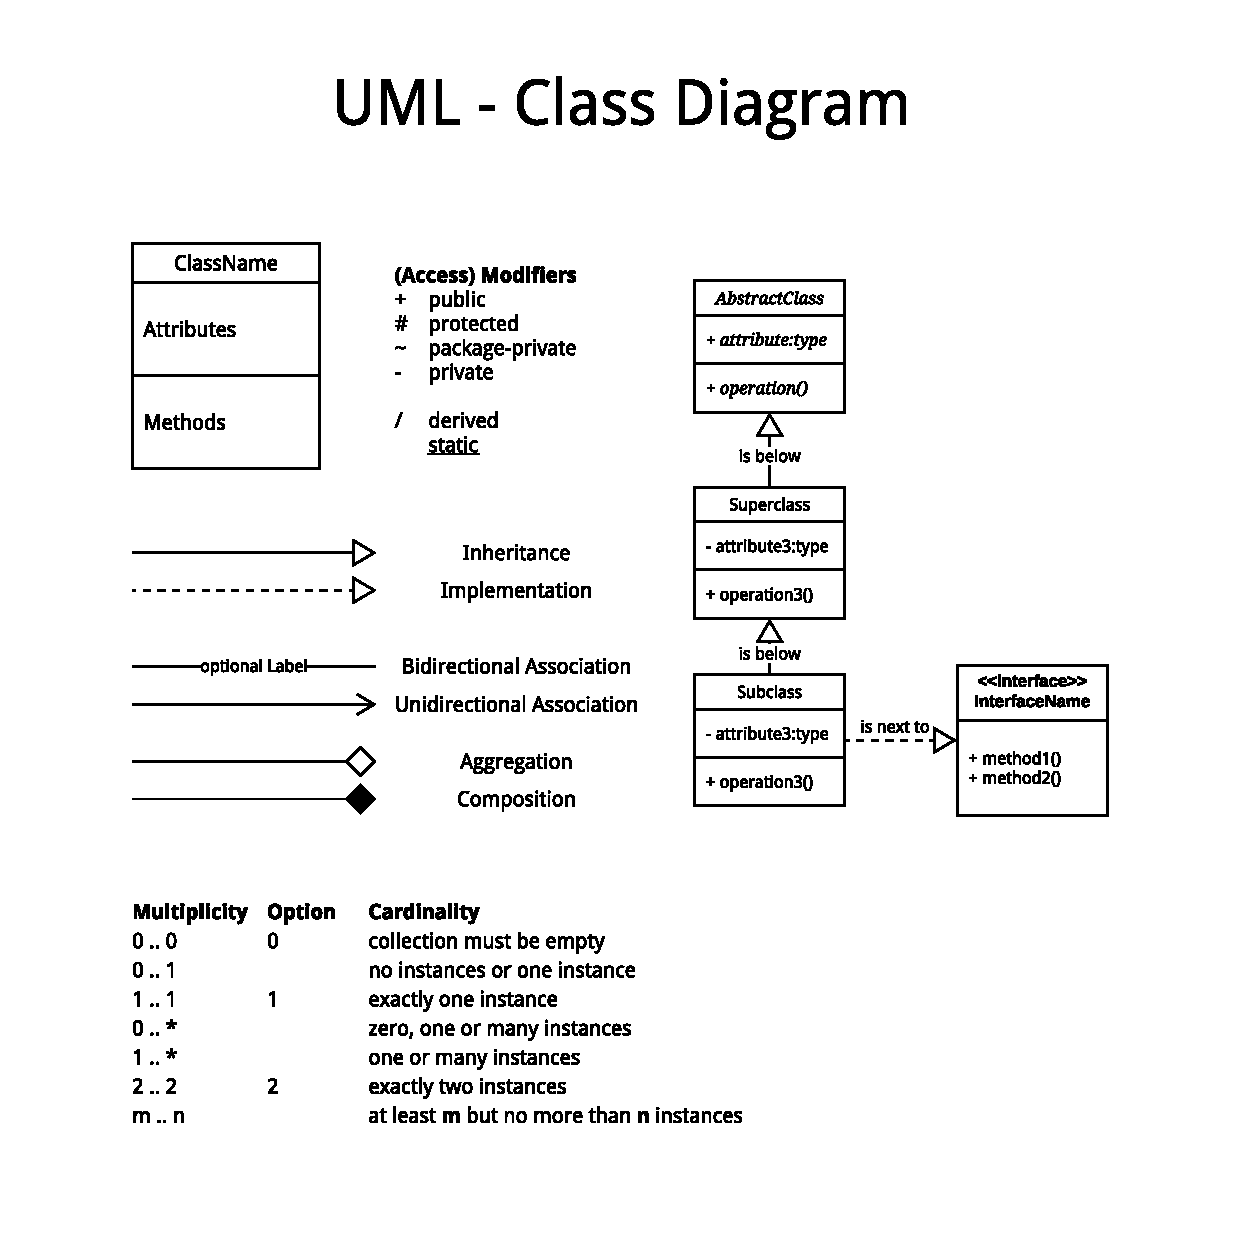
\includegraphics[width=1.3\linewidth]{fig/UML_Classdiagram.pdf}}
        \caption{Klassendiagramm}
        \label{fig:classdiagram}
      \end{figure}
      \newpage

    \subsection{Entity Relationship Diagram, Datenbank}
      \begin{figure}[h!]
        \makebox[\textwidth]{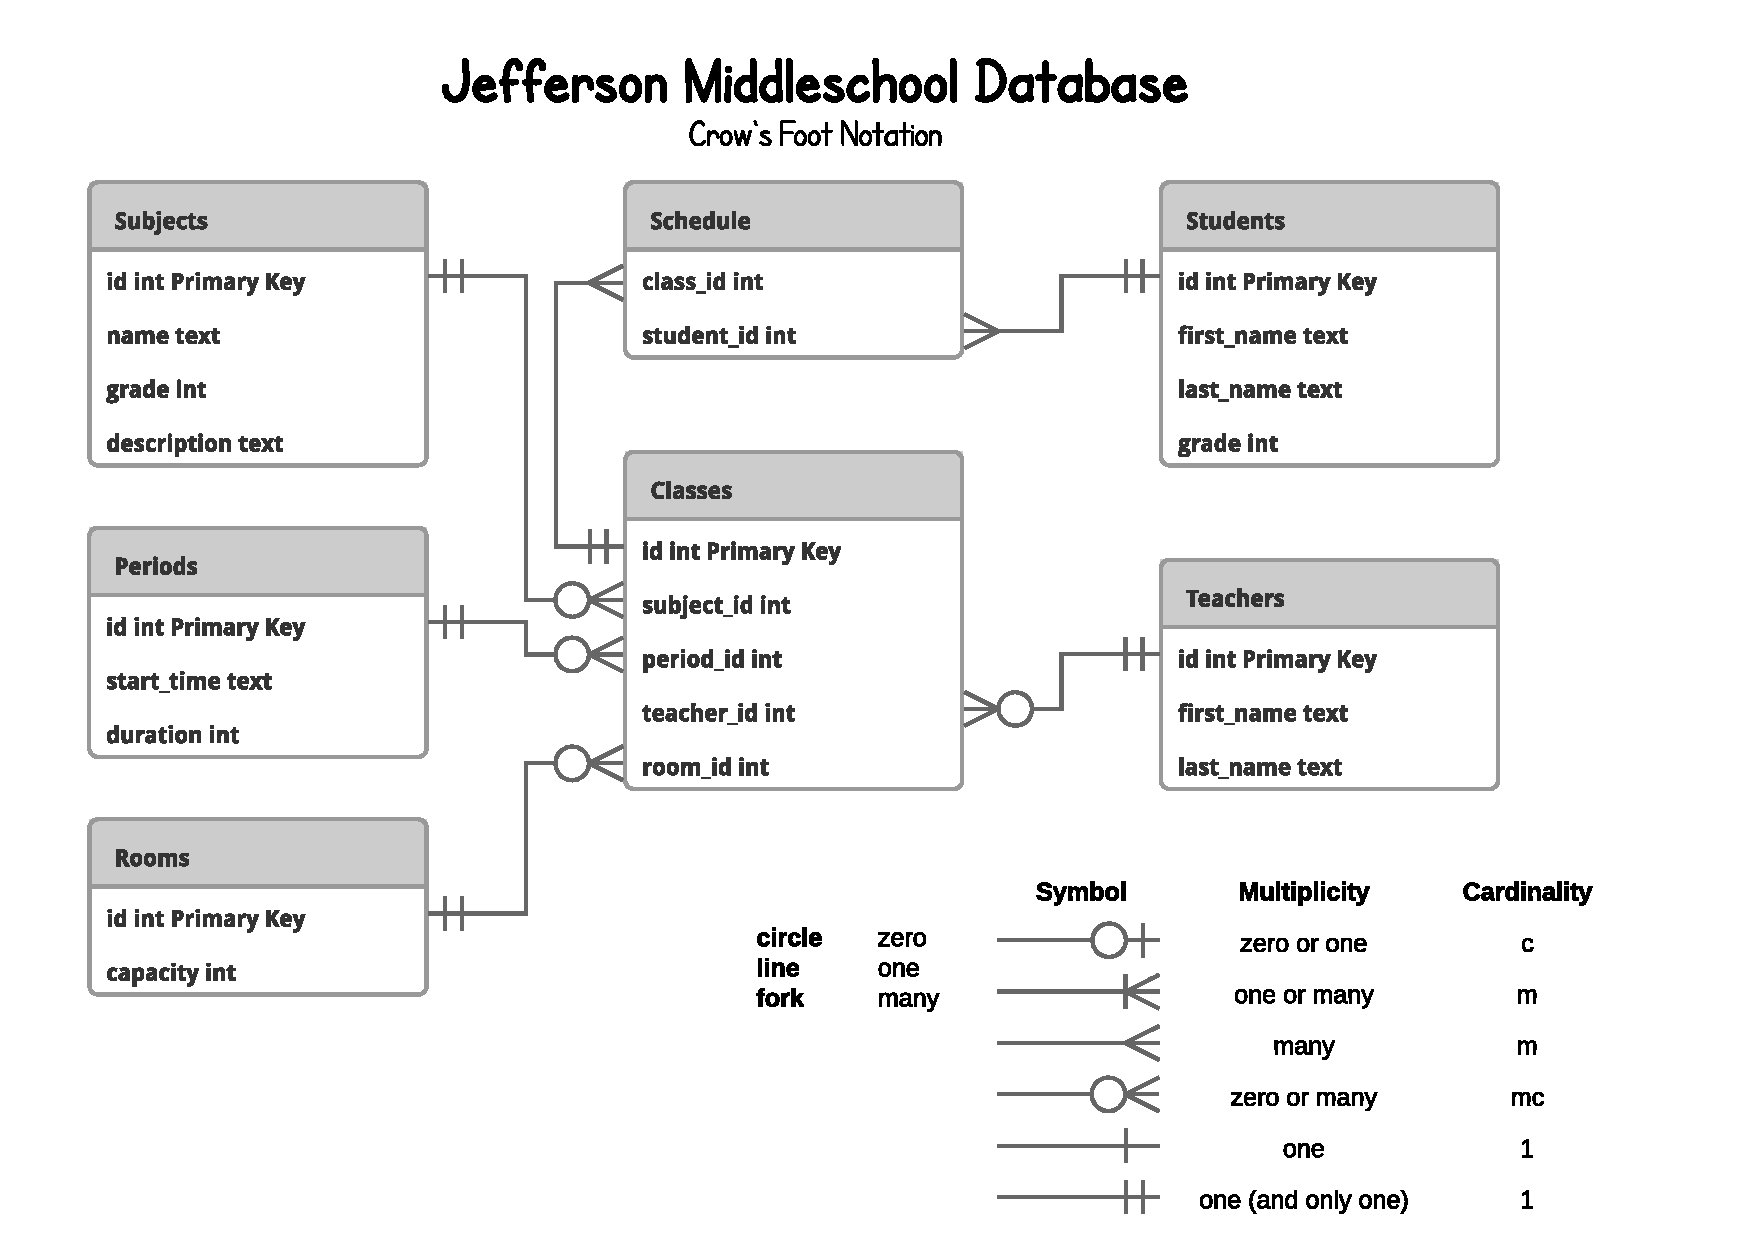
\includegraphics[width=1.3\linewidth]{fig/ERD_JeffersonMiddleSchool.pdf}}
        \caption{Entity Relationship Diagram, Datenbank}
        \label{fig:datadiagram}
      \end{figure}
      \newpage

\end{document}
